% !TeX program = xelatex
\documentclass[a4paper,10pt]{article}

% ============================================================================
% កញ្ចប់បណ្ណាល័យ (Packages) – តាមលំនាំ NGS Preah Krasang (ls_plan.tex)
% ============================================================================
\usepackage[a4paper, left=0.95cm, right=0.95cm, top=0.85cm, bottom=0.92cm, footskip=0.52cm]{geometry}
\usepackage{amsmath}
\usepackage{unicode-math}
\usepackage{fontspec}
\usepackage{array, longtable, multirow, colortbl}
\usepackage[table]{xcolor}
\usepackage{enumitem}
\usepackage{pifont}
\usepackage{fancyhdr}
\usepackage{tikz}
\usetikzlibrary{calc, arrows.meta, angles, quotes, decorations.markings, babel}

% LaTeX 2025 + longtable v4.24 compatibility guard
\makeatletter
\let\@expl@@@mark@update@singlecol@structures@@\relax
\makeatother

% ============================================================================
% ការកំណត់ពុម្ពអក្សរ (Fonts Configuration) – តាមលំនាំស្ដង់ដារ ១០០%
% ============================================================================
% Cross-platform font path resolver (Windows local + Linux/Cloud repo fonts/)
\providecommand{\NGSFindFonts}{%
  \IfFileExists{C:/Windows/Fonts/cambria.ttc}{%
    \def\NGSSysPath{C:/Windows/Fonts/}%
    \def\NGSUserPath{C:/Users/KIT/AppData/Local/Microsoft/Windows/Fonts/}%
  }{%
    \IfFileExists{./fonts/KhmerOSsiemreap.ttf}{\def\NGSSysPath{./fonts/}\def\NGSUserPath{./fonts/}}{%
    \IfFileExists{../fonts/KhmerOSsiemreap.ttf}{\def\NGSSysPath{../fonts/}\def\NGSUserPath{../fonts/}}{%
    \IfFileExists{../../fonts/KhmerOSsiemreap.ttf}{\def\NGSSysPath{../../fonts/}\def\NGSUserPath{../../fonts/}}{%
    \IfFileExists{../../../fonts/KhmerOSsiemreap.ttf}{\def\NGSSysPath{../../../fonts/}\def\NGSUserPath{../../../fonts/}}{%
    \IfFileExists{../../../../fonts/KhmerOSsiemreap.ttf}{\def\NGSSysPath{../../../../fonts/}\def\NGSUserPath{../../../../fonts/}}{%
    \IfFileExists{../../../../../fonts/KhmerOSsiemreap.ttf}{\def\NGSSysPath{../../../../../fonts/}\def\NGSUserPath{../../../../../fonts/}}{%
    \IfFileExists{../../../../../../fonts/KhmerOSsiemreap.ttf}{\def\NGSSysPath{../../../../../../fonts/}\def\NGSUserPath{../../../../../../fonts/}}{%
      \def\NGSSysPath{../../../../../../../fonts/}\def\NGSUserPath{../../../../../../../fonts/}%
    }}}}}}}%
  }%
}
\NGSFindFonts

\setmathfont[
  Path={\NGSSysPath},
  FontIndex=1,
  Scale=1.02
]{cambria.ttc}

\defaultfontfeatures{Ligatures=TeX}

\setmainfont[
  Path={\NGSUserPath},
  Extension=.ttf,
  Script=Khmer,
  BoldFont={KhmerOSsiemreap},
  BoldFeatures={FakeBold=1.8},
  ItalicFont={KhmerOSsiemreap},
  ItalicFeatures={FakeSlant=0.25},
  BoldItalicFont={KhmerOSsiemreap},
  BoldItalicFeatures={FakeBold=1.8, FakeSlant=0.25}
]{KhmerOSsiemreap}

\newfontfamily\muol[
  Path={\NGSUserPath},
  Extension=.ttf,
  Script=Khmer
]{KhmerOSmuollight}

\newfontfamily\TimesEn[
  Path={\NGSSysPath},
  Extension=.ttf,
  Scale=1.00,
  BoldFont={timesbd},
  ItalicFont={timesi},
  BoldItalicFont={timesbi}
]{times}

\newfontfamily\NagaBold[
  Path={\NGSUserPath},
  Extension=.ttf
]{AKbalthom Naga Bold}

\newfontfamily\CalibriFont[
  Path={\NGSSysPath},
  Extension=.ttf
]{calibri}

\newfontfamily\Tacteing[
  Path={\NGSUserPath}
]{TACTENG.TTF}

\newfontfamily\CourierBullet[
  Path={\NGSSysPath},
  Extension=.ttf
]{cour}
\newcommand{\wcirc}{{\CourierBullet\fontsize{9.5pt}{11pt}\selectfont o}}

% ក្បួនកាត់ពាក្យខ្មែរ (Khmer word wrapping)
\XeTeXlinebreaklocale "km"
\XeTeXlinebreakskip = 0pt plus 1pt minus 0.1pt

% ============================================================================
% ការកំណត់ពណ៌ និងទម្រង់ទំព័រ (Colors & Page Style)
% ============================================================================
\definecolor{stepgray}{HTML}{D9D9D9}
\definecolor{headgray}{HTML}{F2F2F2}
\definecolor{boxgray}{HTML}{D9D9D9}
\definecolor{darkred}{HTML}{C00000}
\definecolor{red5e}{HTML}{FF0000}

\pagestyle{fancy}
\fancyhf{}
\renewcommand{\headrulewidth}{0pt}
\fancyfoot[R]{\CalibriFont\fontsize{11pt}{13pt}\selectfont\thepage}

\setlength{\parindent}{0pt}
\setlength{\parskip}{0pt}
\setlength{\tabcolsep}{3.8pt}

\newcolumntype{L}[1]{>{\raggedright\arraybackslash}p{#1}}

% ============================================================================
% ម៉ាក្រូជំនួយ (Helper Macros)
% ============================================================================
\newcommand{\enbf}[1]{{\TimesEn\textbf{#1}}}
\newcommand{\fiveE}[1]{{\NagaBold\fontsize{9.5pt}{13pt}\selectfont\textcolor{red5e}{#1}}}
\newcommand{\timenote}[1]{\textcolor{darkred}{\textit{#1}}}
\newcommand{\redsub}[1]{\textcolor{darkred}{#1}}
\newcommand{\graybox}[1]{\colorbox{boxgray}{\strut\hspace{2pt}#1\hspace{2pt}}}
\newcommand{\ditem}{\tikz[baseline=-0.5ex]\fill (0,0.42ex) -- (0.42ex,0) -- (0,-0.42ex) -- (-0.42ex,0) -- cycle;\hspace{0.3em}}
\newcommand{\cnum}[1]{{\fontsize{10.5pt}{12pt}\selectfont\ding{\numexpr181+#1\relax}}\hspace{0.2em}}
\newcommand{\cfig}[1]{\par\vspace{4pt}{\centering #1\par}\vspace{4pt}}
\newcommand{\stepheader}[1]{\multicolumn{3}{|c|}{\cellcolor{stepgray}\muol #1} \\* \noalign{\hrule height 0.4pt}}
\newcommand{\tri}[1]{\ensuremath{\triangle #1}}
\newcommand{\ang}[1]{\ensuremath{\angle #1}}
\newcommand{\cg}{\ensuremath{\cong}}
\newcommand{\ncg}{\ensuremath{\not\cong}}

% រចនាប័ទ្មគូសសម្គាល់ជ្រុងស្មើគ្នា (Tick mark styles - bold B&W print safe)
\tikzset{
  tk1/.style={postaction={decorate},decoration={markings,mark=at position 0.50 with {\draw[black, line width=0.85pt](0,-0.095)--(0,0.095);}}},
  tk1a/.style={postaction={decorate},decoration={markings,mark=at position 0.30 with {\draw[black, line width=0.85pt](0,-0.095)--(0,0.095);}}},
  tk2/.style={postaction={decorate},decoration={markings,
    mark=at position 0.45 with {\draw[black, line width=0.85pt](0,-0.095)--(0,0.095);},
    mark=at position 0.55 with {\draw[black, line width=0.85pt](0,-0.095)--(0,0.095);}}}
}

% ម៉ាក្រូគូសប្រអប់មុំកែង 90° ត្រង់ B ក្នុងមុំ A-B-C
\newcommand{\rightbox}[4][0.19]{%
  \draw[black, line width=0.8pt]
    ($(#3)!#1!(#2)$) -- ($($(#3)!#1!(#2)$)+($(#3)!#1!(#4)$)-(#3)$) -- ($(#3)!#1!(#4)$);
}

% ក្បាច់ក្រោមបាវចនា (Tacteing Font - Keyboard '3')
\newcommand{\khmflourish}{{\Tacteing\fontsize{36pt}{14pt}\selectfont\raisebox{-5pt}{3}}}

% ============================================================================
% ម៉ាក្រូគូសរូបធរណីមាត្រ (Monochrome B&W TikZ Figures, 100% Black Text)
% ============================================================================

% ១. កំណែកិច្ចការផ្ទះមេរៀនមុន (លំហាត់ #4 & #9)
\newcommand{\figHWold}{%
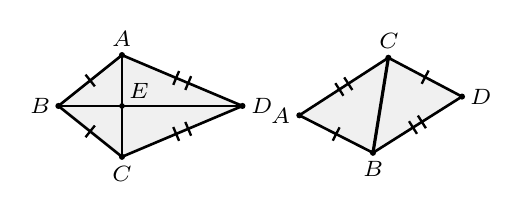
\begin{tikzpicture}[scale=0.85, every node/.style={font=\footnotesize, text=black}]
  % លំហាត់ទី៤ (ខ្លែង ABCD, E ប្រសព្វ AC, BD)
  \begin{scope}[shift={(-1.85,0)}]
    \coordinate (B) at (-0.95, 0);
    \coordinate (A) at (0, 0.76);
    \coordinate (C) at (0, -0.76);
    \coordinate (D) at (1.80, 0);
    \coordinate (E) at (0, 0);
    \fill[gray!12] (A) -- (B) -- (C) -- (D) -- cycle;
    \draw[black, line width=0.95pt, tk1] (A) -- (B);
    \draw[black, line width=0.95pt, tk1] (B) -- (C);
    \draw[black, line width=0.95pt, tk2] (A) -- (D);
    \draw[black, line width=0.95pt, tk2] (C) -- (D);
    \draw[black, line width=0.8pt] (A) -- (C) (B) -- (D);
    \fill[black] (A) circle (1.3pt) node[above=2pt, inner sep=1pt] {$A$};
    \fill[black] (B) circle (1.3pt) node[left=2pt, inner sep=1pt] {$B$};
    \fill[black] (C) circle (1.3pt) node[below=2pt, inner sep=1pt] {$C$};
    \fill[black] (D) circle (1.3pt) node[right=2pt, inner sep=1pt] {$D$};
    \fill[black] (E) circle (1.2pt) node[above right=1.5pt, inner sep=1pt] {$E$};
    \node[anchor=north] at (0.35,-0.92) {លំហាត់ទី៤};
  \end{scope}
  % លំហាត់ទី៩ (ចតុកោណ ABDC, BC រួម)
  \begin{scope}[shift={(1.85,0)}]
    \coordinate (A) at (-1.05, -0.14);
    \coordinate (B) at (0.05, -0.70);
    \coordinate (C) at (0.28, 0.72);
    \coordinate (D) at (1.38, 0.14);
    \fill[gray!12] (A) -- (B) -- (D) -- (C) -- cycle;
    \draw[black, line width=0.95pt, tk1] (A) -- (B);
    \draw[black, line width=0.95pt, tk1] (C) -- (D);
    \draw[black, line width=0.95pt, tk2] (A) -- (C);
    \draw[black, line width=0.95pt, tk2] (B) -- (D);
    \draw[black, line width=1.15pt] (B) -- (C);
    \fill[black] (A) circle (1.3pt) node[left=2pt, inner sep=1pt] {$A$};
    \fill[black] (B) circle (1.3pt) node[below=2pt, inner sep=1pt] {$B$};
    \fill[black] (C) circle (1.3pt) node[above=2pt, inner sep=1pt] {$C$};
    \fill[black] (D) circle (1.3pt) node[right=2pt, inner sep=1pt] {$D$};
    \node[anchor=north] at (0.18,-0.92) {លំហាត់ទី៩};
  \end{scope}
\end{tikzpicture}}

% ២. រំលឹកទី១៖ កែង 90° ឈមអ៊ីប៉ូតេនុស & មុំស្រួចបំពេញ 90° - ∠C
\newcommand{\figPrereqOne}{%
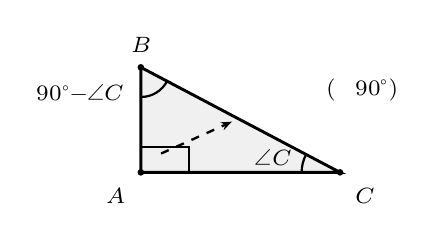
\begin{tikzpicture}[scale=0.92, every node/.style={font=\footnotesize, text=black}]
  \coordinate (A) at (0,0);
  \coordinate (B) at (0,1.45);
  \coordinate (C) at (2.75,0);
  \fill[gray!12] (A) -- (B) -- (C) -- cycle;
  \draw[black, line width=1.05pt] (A) -- (B) -- (C) -- cycle;
  \rightbox[0.24]{B}{A}{C}
  \draw[black, line width=0.85pt, dashed, -{Stealth[length=4pt]}] (0.28,0.26) -- (1.26,0.70);
  \node[above right=2pt] at (1.30,0.78) {អ៊ីប៉ូតេនុស (ឈម $90^\circ$)};
  \draw[black, line width=0.8pt] (0,1.04) arc (-90:-28:0.41);
  \node[left=3pt] at (0,1.10) {$90^\circ{-}\ang{C}$};
  \draw[black, line width=0.8pt] (2.22,0) arc (180:152:0.53);
  \node at (1.82,0.20) {$\ang{C}$};
  \fill[black] (A) circle (1.3pt) node[below left=2pt] {$A$};
  \fill[black] (B) circle (1.3pt) node[above=2pt] {$B$};
  \fill[black] (C) circle (1.3pt) node[below right=2pt] {$C$};
\end{tikzpicture}}

% ៣. រំលឹកទី២៖ ចម្ងាយកែង MA ⊥ OX (ខ្លីបំផុត) vs MD ទ្រេត
\newcommand{\figPrereqTwo}{%
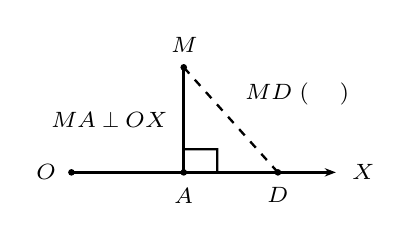
\begin{tikzpicture}[scale=0.92, every node/.style={font=\footnotesize, text=black}]
  \coordinate (O) at (0,0);
  \coordinate (X) at (3.65,0);
  \coordinate (M) at (1.55,1.45);
  \coordinate (A) at (1.55,0);
  \coordinate (D) at (2.85,0);
  \draw[black, line width=1.05pt, -{Stealth[length=4pt]}] (O) -- (X) node[right=2pt] {$X$};
  \draw[black, line width=1.15pt] (M) -- (A) node[midway, left=2.5pt] {$MA \perp OX$};
  \draw[black, line width=0.85pt, dashed] (M) -- (D) node[midway, above right=1.5pt] {$MD$ (ទ្រេត)};
  \rightbox[0.22]{M}{A}{X}
  \fill[black] (O) circle (1.3pt) node[left=2pt] {$O$};
  \fill[black] (M) circle (1.3pt) node[above=2pt] {$M$};
  \fill[black] (A) circle (1.3pt) node[below=2pt] {$A$};
  \fill[black] (D) circle (1.3pt) node[below=2pt] {$D$};
\end{tikzpicture}}

% ៤. E1 Engage: ជម្រាលជណ្ដើរសុវត្ថិភាព (5m, 30°) & ទ្វារទឹកប្រឡាយបំបែក (OX, OY)
\newcommand{\figEngage}{%
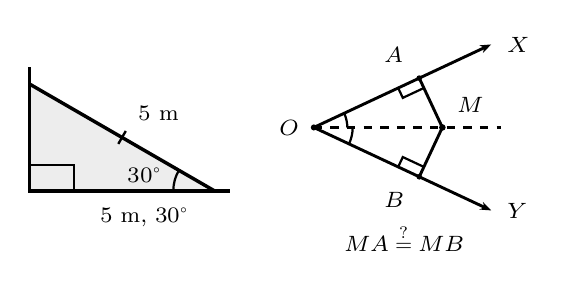
\begin{tikzpicture}[scale=0.85, every node/.style={font=\footnotesize, text=black}]
  % ឆ្វេង៖ ជណ្ដើរជម្រាល 5 m មុំ 30° ផ្អែកជញ្ជាំង 90°
  \begin{scope}[shift={(-3.75, -0.65)}]
    \coordinate (W0) at (0,0);
    \coordinate (W1) at (0,1.60);
    \coordinate (G1) at (2.77,0);
    \fill[gray!14] (W0) -- (W1) -- (G1) -- cycle;
    \draw[black, line width=1.2pt] (0,1.85) -- (W0) -- (3.00,0);
    \draw[black, line width=1.25pt, tk1] (W1) -- (G1) node[midway, above right=2pt] {$5\text{ m}$};
    \rightbox[0.24]{W1}{W0}{G1}
    \draw[black, line width=0.8pt] (2.15,0) arc (180:150:0.62);
    \node at (1.72,0.23) {$30^\circ$};
    \node[below=2pt] at (1.38,-0.02) {ជម្រាល $5\text{ m},\, 30^\circ$};
  \end{scope}
  % ស្ដាំ៖ ទ្វារទឹក M លើពុះមុំប្រឡាយ OX, OY
  \begin{scope}[shift={(0.50, 0.30)}]
    \coordinate (O) at (0,0);
    \coordinate (X) at (2.65, 1.24);
    \coordinate (Y) at (2.65, -1.24);
    \coordinate (M) at (1.92, 0);
    \coordinate (A) at ($(O)!(M)!(X)$);
    \coordinate (B) at ($(O)!(M)!(Y)$);
    \draw[black, line width=1.05pt, -{Stealth[length=4pt]}] (O) -- (X) node[right=2pt] {$X$};
    \draw[black, line width=1.05pt, -{Stealth[length=4pt]}] (O) -- (Y) node[right=2pt] {$Y$};
    \draw[black, line width=0.85pt, dashed] (O) -- (2.80,0);
    \draw[black, line width=1.05pt] (M) -- (A);
    \draw[black, line width=1.05pt] (M) -- (B);
    \rightbox[0.20]{M}{A}{O}
    \rightbox[0.20]{M}{B}{O}
    \draw[black, line width=0.8pt] (0.50,0) arc (0:25:0.50);
    \draw[black, line width=0.8pt] (0.58,0) arc (0:-25:0.58);
    \fill[black] (O) circle (1.3pt) node[left=2pt] {$O$};
    \fill[black] (M) circle (1.4pt) node[above right=2pt] {$M$};
    \fill[black] (A) circle (1.2pt) node[above left=2pt] {$A$};
    \fill[black] (B) circle (1.2pt) node[below left=2pt] {$B$};
    \node[below=4pt] at (1.35,-1.18) {$MA \overset{?}{=} MB$};
  \end{scope}
\end{tikzpicture}}

% ៥. E2 Act 1: ផ្ទាំងកែង 90° + ខ្សែអ៊ីប៉ូតេនុស 5 cm មុំ 35° → ត្រួតរូបបង្វិល ~135°
\newcommand{\figExploreOne}{%
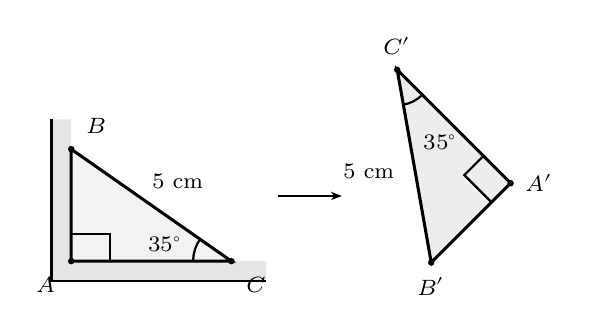
\begin{tikzpicture}[scale=0.90, every node/.style={font=\footnotesize, text=black}]
  % ផ្ទាំងកែង 90° + បន្ទះ 5 cm មុំ 35°
  \begin{scope}[shift={(0,0)}]
    \fill[gray!20] (-0.28,2.00) -- (-0.28,-0.28) -- (2.75,-0.28) -- (2.75,0) -- (0,0) -- (0,2.00) -- cycle;
    \draw[black, line width=0.85pt] (-0.28,2.00) -- (-0.28,-0.28) -- (2.75,-0.28);
    \coordinate (A) at (0,0);
    \coordinate (B) at (0,1.58);
    \coordinate (C) at (2.26,0);
    \fill[gray!10] (A) -- (B) -- (C) -- cycle;
    \draw[black, line width=1.1pt] (A) -- (B) -- (C) -- cycle;
    \rightbox[0.24]{B}{A}{C}
    \draw[black, line width=0.8pt] (1.72,0) arc (180:145:0.54);
    \node at (1.32,0.23) {$35^\circ$};
    \node[above right=1.5pt] at (0.95,0.82) {$5\text{ cm}$};
    \fill[black] (A) circle (1.3pt) node[below left=2pt] {$A$};
    \fill[black] (B) circle (1.3pt) node[above right=2pt] {$B$};
    \fill[black] (C) circle (1.3pt) node[below right=2pt] {$C$};
  \end{scope}
  \draw[black, line width=0.95pt, -{Stealth[length=4pt]}] (2.92,0.92) -- (3.82,0.92) node[midway, above=3pt] {ត្រួត};
  % រូបកាត់បង្វិល ~135°
  \begin{scope}[shift={(4.45,-0.05)}]
    \coordinate (Ap) at (1.75, 1.15);
    \coordinate (Bp) at (0.63, 0.03);
    \coordinate (Cp) at (0.15, 2.75);
    \fill[gray!14] (Ap) -- (Bp) -- (Cp) -- cycle;
    \draw[black, line width=1.1pt] (Ap) -- (Bp) -- (Cp) -- cycle;
    \rightbox[0.24]{Bp}{Ap}{Cp}
    \draw[black, line width=0.8pt] ($(Cp)+(-80:0.50)$) arc (-80:-45:0.50);
    \node at (0.76,1.72) {$35^\circ$};
    \node[left=3pt] at (0.36,1.32) {$5\text{ cm}$};
    \fill[black] (Ap) circle (1.3pt) node[right=2pt] {$A'$};
    \fill[black] (Bp) circle (1.3pt) node[below=2pt] {$B'$};
    \fill[black] (Cp) circle (1.3pt) node[above=2pt] {$C'$};
  \end{scope}
\end{tikzpicture}}

% ៦ក. E2 Act 2 POE 2A: Hyp 5 cm vs Leg 5 cm
\newcommand{\figExplorePOEA}{%
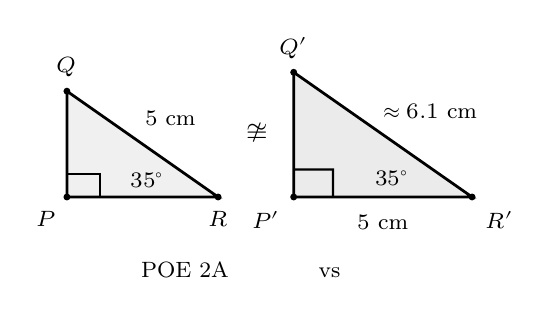
\begin{tikzpicture}[scale=0.96, every node/.style={font=\footnotesize, text=black}]
  \coordinate (P) at (0,0);
  \coordinate (Q) at (0,1.40);
  \coordinate (R) at (2.00,0);
  \fill[gray!12] (P) -- (Q) -- (R) -- cycle;
  \draw[black, line width=1.0pt] (P) -- (Q) -- (R) -- cycle;
  \rightbox[0.22]{Q}{P}{R}
  \node[above right=1.5pt] at (0.85,0.75) {$5\text{ cm}$};
  \node at (1.06,0.22) {$35^\circ$};
  \fill[black] (P) circle (1.3pt) node[below left=1.5pt] {$P$};
  \fill[black] (Q) circle (1.3pt) node[above=1.5pt] {$Q$};
  \fill[black] (R) circle (1.3pt) node[below=1.5pt] {$R$};
  \node[font=\normalsize] at (2.52, 0.85) {$\ncg$};
  \coordinate (Pp) at (3.00,0);
  \coordinate (Qp) at (3.00,1.65);
  \coordinate (Rp) at (5.36,0);
  \fill[gray!16] (Pp) -- (Qp) -- (Rp) -- cycle;
  \draw[black, line width=1.0pt] (Pp) -- (Qp) -- (Rp) -- cycle;
  \rightbox[0.22]{Qp}{Pp}{Rp}
  \node[below=3pt] at (4.18,0) {$5\text{ cm}$};
  \node[above right=1.5pt] at (4.00,0.85) {$\approx 6.1\text{ cm}$};
  \node at (4.30,0.24) {$35^\circ$};
  \fill[black] (Pp) circle (1.3pt) node[below left=1.5pt] {$P'$};
  \fill[black] (Qp) circle (1.3pt) node[above=1.5pt] {$Q'$};
  \fill[black] (Rp) circle (1.3pt) node[below right=1.5pt] {$R'$};
  \node[below=15pt] at (2.68,-0.18) {POE 2A៖ អ៊ីប៉ូតេនុស vs ជ្រុងកែង};
\end{tikzpicture}}

% ៦ខ. E2 Act 2 POE 2B: Fold OM & Slanted MD
\newcommand{\figExplorePOEB}{%
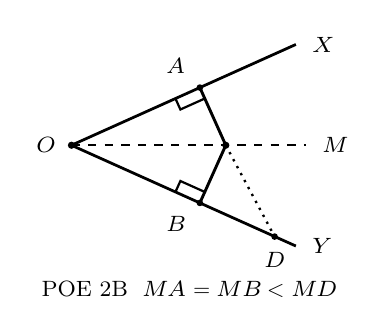
\begin{tikzpicture}[scale=1.00, every node/.style={font=\footnotesize, text=black}]
  \coordinate (O) at (0,0);
  \coordinate (X) at (2.85, 1.28);
  \coordinate (Y) at (2.85, -1.28);
  \coordinate (M) at (1.96, 0);
  \coordinate (A) at ($(O)!(M)!(X)$);
  \coordinate (B) at ($(O)!(M)!(Y)$);
  \coordinate (D) at (2.58, -1.16);
  \draw[black, line width=1.0pt] (O) -- (X) node[right=2pt] {$X$};
  \draw[black, line width=1.0pt] (O) -- (Y) node[right=2pt] {$Y$};
  \draw[black, line width=0.9pt, dashed] (O) -- (2.98,0) node[right=2pt] {$M$};
  \draw[black, line width=1.05pt] (M) -- (A);
  \draw[black, line width=1.05pt] (M) -- (B);
  \draw[black, line width=0.85pt, dotted] (M) -- (D);
  \rightbox[0.19]{M}{A}{O}
  \rightbox[0.19]{M}{B}{O}
  \fill[black] (O) circle (1.3pt) node[left=2pt] {$O$};
  \fill[black] (M) circle (1.3pt);
  \fill[black] (A) circle (1.2pt) node[above left=1.5pt] {$A$};
  \fill[black] (B) circle (1.2pt) node[below left=1.5pt] {$B$};
  \fill[black] (D) circle (1.2pt) node[below=2pt] {$D$};
  \node[below=10pt] at (1.50,-1.24) {POE 2B៖ $MA=MB < MD$};
\end{tikzpicture}}

% ៧. E3 Explain: ទ្រឹស្ដីបទ អ.ម (HA) បង្វិល ~135° & ព្រួញឈម 90°
\newcommand{\figThmHA}{%
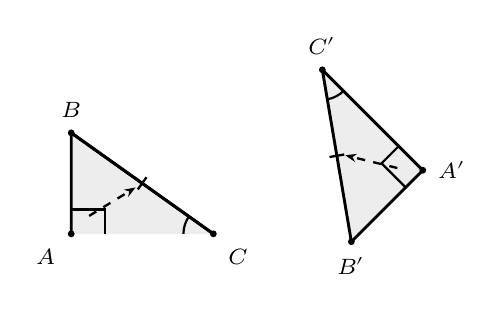
\begin{tikzpicture}[scale=0.95, every node/.style={font=\footnotesize, text=black}]
  % ត្រីកោណទី១
  \coordinate (A) at (0,0);
  \coordinate (B) at (0,1.35);
  \coordinate (C) at (1.90,0);
  \fill[gray!14] (A) -- (B) -- (C) -- cycle;
  \draw[black, line width=1.05pt] (A) -- (B) -- (C);
  \draw[black, line width=1.05pt, tk1] (B) -- (C);
  \rightbox[0.24]{B}{A}{C}
  \draw[black, line width=0.85pt, dashed, -{Stealth[length=4pt]}] (0.24,0.24) -- (0.86,0.62);
  \draw[black, line width=0.8pt] (1.50,0) arc (180:144.6:0.40);
  \fill[black] (A) circle (1.3pt) node[below left=2pt] {$A$};
  \fill[black] (B) circle (1.3pt) node[above=2pt] {$B$};
  \fill[black] (C) circle (1.3pt) node[below right=2pt] {$C$};
  % ត្រីកោណទី២ បង្វិល 135°
  \coordinate (Ap) at (4.70, 0.85);
  \coordinate (Bp) at (3.745, -0.105);
  \coordinate (Cp) at (3.357, 2.193);
  \fill[gray!14] (Ap) -- (Bp) -- (Cp) -- cycle;
  \draw[black, line width=1.05pt] (Ap) -- (Bp) (Ap) -- (Cp);
  \draw[black, line width=1.05pt, tk1] (Bp) -- (Cp);
  \rightbox[0.24]{Bp}{Ap}{Cp}
  \draw[black, line width=0.85pt, dashed, -{Stealth[length=4pt]}]
    (4.36, 0.88) -- ($(Bp)!0.52!(Cp)+(0.12,-0.04)$);
  \draw[black, line width=0.8pt] ($(Cp)+(-79.6:0.40)$) arc (-79.6:-44.6:0.40);
  \fill[black] (Ap) circle (1.3pt) node[right=2pt] {$A'$};
  \fill[black] (Bp) circle (1.3pt) node[below=2pt] {$B'$};
  \fill[black] (Cp) circle (1.3pt) node[above=2pt] {$C'$};
\end{tikzpicture}}

% ៨. E4 Elaborate: លំហាត់គំរូ (ទំព័រ ១៥៣) — ហាមគូស / លើ OA, OB ជាដាច់ខាត!
\newcommand{\figModelHA}{%
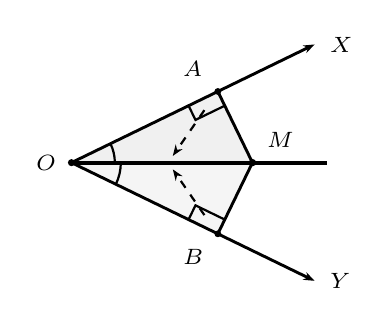
\begin{tikzpicture}[scale=0.95, every node/.style={font=\footnotesize, text=black}]
  \coordinate (O) at (0,0);
  \coordinate (X) at (3.25, 1.58);
  \coordinate (Y) at (3.25, -1.58);
  \coordinate (M) at (2.42, 0);
  \coordinate (A) at ($(O)!(M)!(X)$);
  \coordinate (B) at ($(O)!(M)!(Y)$);
  \fill[gray!12] (O) -- (A) -- (M) -- cycle;
  \fill[gray!8] (O) -- (B) -- (M) -- cycle;
  \draw[black, line width=1.05pt, -{Stealth[length=4pt]}] (O) -- (X) node[right=2pt] {$X$};
  \draw[black, line width=1.05pt, -{Stealth[length=4pt]}] (O) -- (Y) node[right=2pt] {$Y$};
  \draw[black, line width=1.35pt] (O) -- (3.42,0);
  \draw[black, line width=1.05pt] (M) -- (A);
  \draw[black, line width=1.05pt] (M) -- (B);
  \rightbox[0.20]{M}{A}{O}
  \rightbox[0.20]{M}{B}{O}
  % ព្រួញឈម 90° ចង្អុលទៅអ៊ីប៉ូតេនុសរួម OM
  \draw[black, line width=0.8pt, dashed, -{Stealth[length=4pt]}] ($(A)+(-0.18,-0.25)$) -- ($(O)!0.56!(M)+(0,0.09)$);
  \draw[black, line width=0.8pt, dashed, -{Stealth[length=4pt]}] ($(B)+(-0.18,0.25)$) -- ($(O)!0.56!(M)+(0,-0.09)$);
  % ធ្នូមុំពុះស្មើគ្នាត្រង់ O
  \draw[black, line width=0.8pt] (0.58,0) arc (0:26:0.58);
  \draw[black, line width=0.8pt] (0.66,0) arc (0:-26:0.66);
  \fill[black] (O) circle (1.35pt) node[left=2pt] {$O$};
  \fill[black] (A) circle (1.3pt) node[above left=2pt] {$A$};
  \fill[black] (B) circle (1.3pt) node[below left=2pt] {$B$};
  \fill[black] (M) circle (1.4pt) node[above right=2pt] {$M$};
\end{tikzpicture}}

% ៩. E5 Evaluate: ប្រតិបត្តិ (ទំព័រ ១៥៤) — រូបគោល ΔABC (លើ) + រូបបំបែក ΔADB & ΔAEC (ក្រោម)
\newcommand{\figPracticeHA}{%
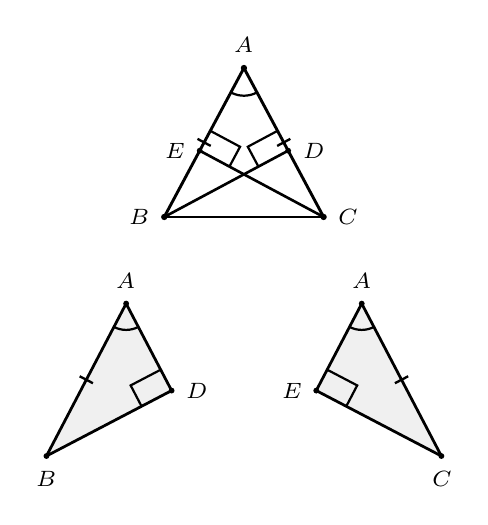
\begin{tikzpicture}[scale=0.88, every node/.style={font=\footnotesize, text=black}]
  % រូបគោល ΔABC (AB=AC, BD⊥AC, CE⊥AB)
  \begin{scope}[shift={(0, 3.45)}]
    \coordinate (A) at (0, 2.15);
    \coordinate (B) at (-1.15, 0);
    \coordinate (C) at (1.15, 0);
    \coordinate (D) at ($(A)!(B)!(C)$);
    \coordinate (E) at ($(A)!(C)!(B)$);
    \draw[black, line width=1.05pt, tk1] (A) -- (B);
    \draw[black, line width=1.05pt, tk1] (A) -- (C);
    \draw[black, line width=1.05pt] (B) -- (C);
    \draw[black, line width=0.95pt] (B) -- (D);
    \draw[black, line width=0.95pt] (C) -- (E);
    \rightbox[0.24]{B}{D}{A}
    \rightbox[0.24]{C}{E}{A}
    \draw[black, line width=0.8pt] ($(A)+(-117:0.40)$) arc (-117:-63:0.40);
    \fill[black] (A) circle (1.3pt) node[above=2pt] {$A$};
    \fill[black] (B) circle (1.3pt) node[left=2pt] {$B$};
    \fill[black] (C) circle (1.3pt) node[right=2pt] {$C$};
    \fill[black] (D) circle (1.2pt) node[right=2pt] {$D$};
    \fill[black] (E) circle (1.2pt) node[left=2pt] {$E$};
  \end{scope}
  % បំបែក ΔADB & ΔAEC នៅជួរក្រោម
  \begin{scope}[shift={(-1.70, 0)}]
    \coordinate (A1) at (0, 2.20);
    \coordinate (B1) at (-1.15, 0);
    \coordinate (C1) at (1.15, 0);
    \coordinate (D1) at ($(A1)!(B1)!(C1)$);
    \fill[gray!12] (A1) -- (D1) -- (B1) -- cycle;
    \draw[black, line width=1.0pt, tk1] (A1) -- (B1);
    \draw[black, line width=1.0pt] (A1) -- (D1) -- (B1);
    \rightbox[0.24]{B1}{D1}{A1}
    \draw[black, line width=0.8pt] ($(A1)+(-117:0.38)$) arc (-117:-63:0.38);
    \fill[black] (A1) circle (1.2pt) node[above=2pt] {$A$};
    \fill[black] (D1) circle (1.2pt) node[right=2pt] {$D$};
    \fill[black] (B1) circle (1.2pt) node[below=2pt] {$B$};
  \end{scope}
  \begin{scope}[shift={(1.70, 0)}]
    \coordinate (A2) at (0, 2.20);
    \coordinate (B2) at (-1.15, 0);
    \coordinate (C2) at (1.15, 0);
    \coordinate (E2) at ($(A2)!(C2)!(B2)$);
    \fill[gray!12] (A2) -- (E2) -- (C2) -- cycle;
    \draw[black, line width=1.0pt, tk1] (A2) -- (C2);
    \draw[black, line width=1.0pt] (A2) -- (E2) -- (C2);
    \rightbox[0.24]{C2}{E2}{A2}
    \draw[black, line width=0.8pt] ($(A2)+(-117:0.38)$) arc (-117:-63:0.38);
    \fill[black] (A2) circle (1.2pt) node[above=2pt] {$A$};
    \fill[black] (E2) circle (1.2pt) node[left=2pt] {$E$};
    \fill[black] (C2) circle (1.2pt) node[below=2pt] {$C$};
  \end{scope}
\end{tikzpicture}}

% ១០. E5 Evaluate: រូបសង្ខេបកាតត្រួតពិនិត្យ A-B & C-D (បំបែកជា ២ ជួរច្បាស់)
\newcommand{\figExitCardsHAab}{%
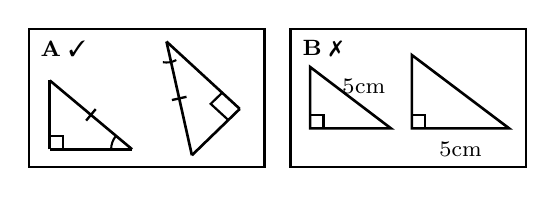
\begin{tikzpicture}[scale=0.95, every node/.style={font=\footnotesize, text=black}]
  % កាត A: អ.ម បង្វិល ~135° ✓
  \begin{scope}[shift={(0, 0)}]
    \draw[black, line width=0.85pt] (0,0) rectangle (3.15,1.85);
    \node[anchor=north west, inner sep=3pt] at (0.04,1.81) {\textbf{A} \ding{51}};
    \draw[black, line width=0.95pt] (0.28,0.24) -- (0.28,1.16);
    \draw[black, line width=0.95pt] (0.28,0.24) -- (1.38,0.24);
    \draw[black, line width=0.95pt, tk1] (0.28,1.16) -- (1.38,0.24);
    \draw[black, line width=0.8pt] (0.28,0.42) -- (0.46,0.42) -- (0.46,0.24);
    \draw[black, line width=0.75pt] (1.10,0.24) arc (180:140:0.28);
    \coordinate (Ap) at (2.82,0.78);
    \coordinate (Bp) at (2.18,0.16);
    \coordinate (Cp) at (1.84,1.68);
    \draw[black, line width=0.95pt] (Ap) -- (Bp) (Ap) -- (Cp);
    \draw[black, line width=0.95pt, tk1] (Bp) -- (Cp);
    \rightbox[0.24]{Bp}{Ap}{Cp}
    \draw[black, line width=0.75pt] ($(Cp)+(-62:0.28)$) arc (-62:-100:0.28);
  \end{scope}
  % កាត B: Hyp vs Leg 5 cm ✗
  \begin{scope}[shift={(3.50, 0)}]
    \draw[black, line width=0.85pt] (0,0) rectangle (3.15,1.85);
    \node[anchor=north west, inner sep=3pt] at (0.04,1.81) {\textbf{B} \ding{55}};
    \draw[black, line width=0.95pt] (0.26,0.52) -- (0.26,1.34) -- (1.34,0.52) -- cycle;
    \draw[black, line width=0.8pt] (0.26,0.70) -- (0.44,0.70) -- (0.44,0.52);
    \node at (0.98,1.08) {$5\text{cm}$};
    \draw[black, line width=0.95pt] (1.62,0.52) -- (1.62,1.50) -- (2.92,0.52) -- cycle;
    \draw[black, line width=0.8pt] (1.62,0.70) -- (1.80,0.70) -- (1.80,0.52);
    \node at (2.27,0.24) {$5\text{cm}$};
  \end{scope}
\end{tikzpicture}}
\newcommand{\figExitCardsHAcd}{%
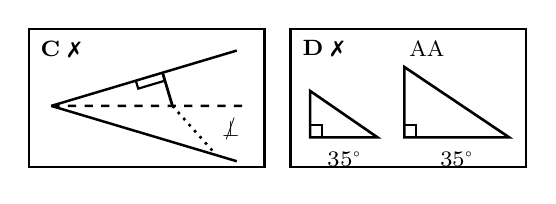
\begin{tikzpicture}[scale=0.95, every node/.style={font=\footnotesize, text=black}]
  % កាត C: ទ្រេតមិនកែង MD ✗
  \begin{scope}[shift={(0, 0)}]
    \draw[black, line width=0.85pt] (0,0) rectangle (3.15,1.85);
    \node[anchor=north west, inner sep=3pt] at (0.04,1.81) {\textbf{C} \ding{55}};
    \coordinate (Oc) at (0.30,0.82);
    \coordinate (Xc) at (2.78,1.56);
    \coordinate (Yc) at (2.78,0.08);
    \coordinate (Mc) at (1.92,0.82);
    \coordinate (Ac) at ($(Oc)!(Mc)!(Xc)$);
    \coordinate (Dc) at (2.50,0.17);
    \draw[black, line width=0.9pt] (Oc) -- (Xc) (Oc) -- (Yc);
    \draw[black, line width=0.85pt, dashed] (Oc) -- (2.86,0.82);
    \draw[black, line width=1.0pt] (Mc) -- (Ac);
    \draw[black, line width=0.95pt, dotted] (Mc) -- (Dc);
    \rightbox[0.24]{Mc}{Ac}{Oc}
    \node at (2.70,0.54) {$\not\perp$};
  \end{scope}
  % កាត D: AA 90°, 35° គ្មានអ៊ីប៉ូតេនុស ✗
  \begin{scope}[shift={(3.50, 0)}]
    \draw[black, line width=0.85pt] (0,0) rectangle (3.15,1.85);
    \node[anchor=north west, inner sep=3pt] at (0.04,1.81) {\textbf{D} \ding{55}};
    \node[anchor=north east, inner sep=3pt] at (3.11,1.81) {AA គ្មានជ្រុង};
    \draw[black, line width=0.95pt] (0.26,0.40) -- (0.26,1.02) -- (1.16,0.40) -- cycle;
    \draw[black, line width=0.8pt] (0.26,0.56) -- (0.42,0.56) -- (0.42,0.40);
    \node[below=1pt] at (0.72,0.38) {$35^\circ$};
    \draw[black, line width=0.95pt] (1.52,0.40) -- (1.52,1.34) -- (2.92,0.40) -- cycle;
    \draw[black, line width=0.8pt] (1.52,0.56) -- (1.68,0.56) -- (1.68,0.40);
    \node[below=1pt] at (2.22,0.38) {$35^\circ$};
  \end{scope}
\end{tikzpicture}}

% ១១. ជំហានទី៥ កិច្ចការផ្ទះ៖ លំហាត់ទី៦ (ទំ.១៦៤) & លំហាត់ទី៧ (ទំ.១៦៥)
\newcommand{\figHWnewHA}{%
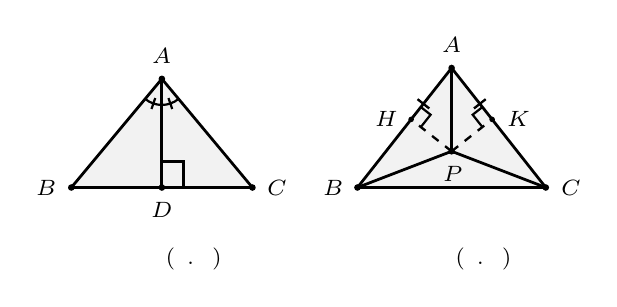
\begin{tikzpicture}[scale=0.92, every node/.style={font=\footnotesize, text=black}]
  % លំហាត់ទី៦ (AD ជាជ្រុងកែងរួម, ម.ជ.ម)
  \begin{scope}[shift={(-2.05,0)}]
    \coordinate (A) at (0, 1.50);
    \coordinate (B) at (-1.25, 0);
    \coordinate (C) at (1.25, 0);
    \coordinate (D) at (0, 0);
    \fill[gray!10] (A) -- (B) -- (C) -- cycle;
    \draw[black, line width=1.0pt] (A) -- (B) -- (C) -- cycle;
    \draw[black, line width=1.15pt] (A) -- (D);
    \rightbox[0.24]{A}{D}{C}
    \draw[black, line width=0.8pt] ($(A)+(-129.6:0.36)$) arc (-129.6:-50.4:0.36);
    \draw[black, line width=0.8pt] ($(A)+(-109:0.28)$) -- ($(A)+(-109:0.44)$);
    \draw[black, line width=0.8pt] ($(A)+(-71:0.28)$) -- ($(A)+(-71:0.44)$);
    \fill[black] (A) circle (1.3pt) node[above=2pt] {$A$};
    \fill[black] (B) circle (1.3pt) node[left=2pt] {$B$};
    \fill[black] (C) circle (1.3pt) node[right=2pt] {$C$};
    \fill[black] (D) circle (1.3pt) node[below=2pt] {$D$};
    \node[below=14pt] at (0,-0.16) {លំហាត់ទី៦ (ទំ.១៦៤)};
  \end{scope}
  % លំហាត់ទី៧ (P លើពុះមុំ A, ក. PB=PC, ខ. PH⊥AB, PK⊥AC)
  \begin{scope}[shift={(1.95,0)}]
    \coordinate (A) at (0, 1.65);
    \coordinate (B) at (-1.30, 0);
    \coordinate (C) at (1.30, 0);
    \coordinate (P) at (0, 0.50);
    \coordinate (H) at ($(A)!(P)!(B)$);
    \coordinate (K) at ($(A)!(P)!(C)$);
    \fill[gray!10] (A) -- (B) -- (C) -- cycle;
    \draw[black, line width=1.0pt, tk1a] (A) -- (B);
    \draw[black, line width=1.0pt, tk1a] (A) -- (C);
    \draw[black, line width=1.0pt] (B) -- (C) (B) -- (P) -- (C);
    \draw[black, line width=0.9pt] (A) -- (P);
    \draw[black, line width=0.85pt, dashed] (P) -- (H) (P) -- (K);
    \rightbox[0.24]{P}{H}{A}
    \rightbox[0.24]{P}{K}{A}
    \fill[black] (A) circle (1.3pt) node[above=2pt] {$A$};
    \fill[black] (B) circle (1.3pt) node[left=2pt] {$B$};
    \fill[black] (C) circle (1.3pt) node[right=2pt] {$C$};
    \fill[black] (P) circle (1.3pt) node[below=2pt] {$P$};
    \fill[black] (H) circle (1.1pt) node[left=2pt] {$H$};
    \fill[black] (K) circle (1.1pt) node[right=2pt] {$K$};
    \node[below=14pt] at (0,-0.16) {លំហាត់ទី៧ (ទំ.១៦៥)};
  \end{scope}
\end{tikzpicture}}

% ============================================================================
% ចាប់ផ្ដើមឯកសារ (Document Body)
% ============================================================================
\begin{document}
\fontsize{10pt}{15.2pt}\selectfont

% -------------------- ក្បាលកិច្ចតែងការ (Header) --------------------
\begin{center}
  {\muol\fontsize{11pt}{16pt}\selectfont ព្រះរាជាណាចក្រកម្ពុជា}\\[2pt]
  {\muol\fontsize{10pt}{15pt}\selectfont ជាតិ សាសនា ព្រះមហាក្សត្រ}\\[1pt]
  \khmflourish
\end{center}

\vspace{-19pt}
{\muol\fontsize{9.5pt}{13.2pt}\selectfont
មន្ទីរអប់រំ យុវជន និងកីឡា ខេត្តកំពង់ធំ\\
ការិយាល័យអប់រំ យុវជន និងកីឡា ស្រុកកំពង់ស្វាយ\\
អនុវិទ្យាល័យព្រះក្រសាំង}

\vspace{-1pt}
\begin{center}
  {\muol\fontsize{10pt}{15pt}\selectfont កិច្ចតែងការបង្រៀន}
\end{center}
\vspace{0pt}

% -------------------- ព័ត៌មានទូទៅ (Metadata) --------------------
{\renewcommand{\arraystretch}{1.00}
\hspace*{4.6cm}%
\begin{tabular}{@{}l l l@{}}
  - \hspace{0.35cm} មុខវិជ្ជា & : & គណិតវិទ្យា ថ្នាក់ទី៨ \\
  - \hspace{0.35cm} ចំណងជើងមេរៀន & : & មេរៀនទី១២ ការប្រៀបធៀបត្រីកោណ \\
  - \hspace{0.35cm} ចំណងជើងរង & : & ១.៣. លក្ខខណ្ឌចំពោះត្រីកោណកែងប៉ុនគ្នា \\
  & & ១.៣.១ អ៊ីប៉ូតេនុសប៉ុនគ្នា និងមុំស្រួចមួយប៉ុនគ្នា (អ.ម) និងលក្ខណៈពុះមុំ \\
  - \hspace{0.35cm} រយៈពេល & : & ១ ម៉ោងសិក្សា (៥០នាទី) \\
  - \hspace{0.35cm} បង្រៀនដោយ & : & ហុក ប៊ុនថែន \\
  - \hspace{0.35cm} កាលបរិច្ឆេទ & : & ថ្ងៃសៅរ៍ ទី២៨ ខែវិច្ឆិកា ឆ្នាំ២០២៦ \\
\end{tabular}

\vspace{1pt}

% -------------------- I. វត្ថុបំណង --------------------
\textbf{I.} {\muol វត្ថុបំណង}\\[1pt]
\hspace*{0.55cm}%
\begin{tabular}{@{}l l l@{}}
  \wcirc \hspace{0.25cm} វិជ្ជាសម្បទា & : & សិស្សកំណត់បានពីលក្ខខណ្ឌត្រីកោណកែងប៉ុនគ្នា អ.ម (HA) តាមពិសោធន៍ផ្ទាំងកែង $90^\circ$ អ៊ីប៉ូតេនុស $5\text{cm}$ \\
  & & មុំ $35^\circ$ បង្ហាញសម្រាយ $90^\circ{-}\ang{C}\to$ ម.ជ.ម (កែ $\ang{B}=\ang{B'}$) និងពំនោលលក្ខណៈពុះមុំ (ផ្ទាល់-ច្រាស) ។ \\
  \wcirc \hspace{0.25cm} បំណិនសម្បទា & : & សិស្សបត់ក្រដាសបង្កើតពុះមុំ ប្រើព្រួញឈម $90^\circ$ \textbf{[tracing]} ធនាគារហេតុផល \cnum{1}--\cnum{5} និងបំបែកត្រីកោណត្រួតគ្នា \\
  & & $\tri{ADB}, \tri{AEC}$ ដើម្បីស្រាយបញ្ជាក់ និងបែងចែកករណី អ.ម (HA) ពីជ្រុងកែងស្មើ (LA) ឬមុំដូចគ្នា (AA) ។ \\
  \wcirc \hspace{0.25cm} ចរិយាសម្បទា & : & សិស្សសហការជា «ក្រុមស្ថាបត្យករជណ្ដើរសុវត្ថិភាព» ហ៊ានទស្សន៍ទាយដោយភស្តុតាង និងមិនបន្ថែម \\
  & & សញ្ញាស្មើ \textbf{/} មុនការសន្និដ្ឋាន ប្រកបដោយភាពប្រុងប្រយ័ត្ន និងទំនួលខុសត្រូវ ។ \\
\end{tabular}

\vspace{1pt}

% -------------------- II. សម្ភារៈឧបទេស --------------------
\textbf{II.} {\muol សម្ភារៈឧបទេស}\\[1pt]
\hspace*{0.55cm}$\bullet$ \hspace{0.35cm} សៀវភៅគោលទី៨ (ទំ.១៥៣--១៥៤, ១៦៤--១៦៥) កែង $90^\circ$ រ៉ាព័រទ័រ កញ្ចប់កាត់ ១:១ (ទំព័រ ១) កាត E4--E5 ផ្ទាំង \cnum{1}--\cnum{5} កាត A--D (ស-ខ្មៅ)

\vspace{1pt}

% -------------------- III. វិធីសាស្រ្តបង្រៀន --------------------
\textbf{III.} {\muol វិធីសាស្រ្តបង្រៀន}\\[1pt]
\hspace*{0.55cm}%
\begin{tabular}{@{}l l l@{}}
  $\bullet$ \hspace{0.35cm} គោលវិធី & : \hspace{0.7cm} & សិស្សមជ្ឈមណ្ឌល \\
  $\bullet$ \hspace{0.35cm} យុទ្ធវិធីបង្រៀន & : & ស្ថាបនានិយម គម្រូ 5Es (ពិសោធន៍ ១:១ បត់ POE ព្រួញ $90^\circ$ \textbf{[tracing]} \& ស្ទូឌីយោ ៣ តួនាទី) \\
\end{tabular}
}

\vspace{1pt}

% -------------------- IV. ដំណើរការបង្រៀន --------------------
\textbf{IV.} {\muol ដំណើរការបង្រៀន}

% ============================================================================
% តារាងដំណើរការបង្រៀន (Modular Multi-Row 3-Column Table – 50 នាទី)
% ============================================================================
\renewcommand{\arraystretch}{1.15}
\begin{longtable}{|L{5.50cm}|L{7.90cm}|L{4.80cm}|}
\hline
\rowcolor{headgray}
\multicolumn{1}{|c|}{\muol សកម្មភាពគ្រូ} &
\multicolumn{1}{c|}{\muol ខ្លឹមសារមេរៀន} &
\multicolumn{1}{c|}{\muol សកម្មភាពសិស្ស} \\
\hline
\endfirsthead

\hline
\endhead

\hline
\endfoot

\hline
\endlastfoot

% ==================== ជំហានទី១ (2min) ====================
\stepheader{ជំហានទី១ \enbf{(}រដ្ឋបាលថ្នាក់\enbf{)}}
- ពិនិត្យអវត្តមាន និងអនាម័យថ្នាក់រៀន \newline
- ចាត់សិស្សជាក្រុម ៣ នាក់ («ក្រុមស្ថាបត្យករជណ្ដើរសុវត្ថិភាព») \newline
- ចែកសន្លឹកកិច្ចការទំព័រ ១ (១:១) ទុកលើតុ
&
\hspace*{0.3cm}- រដ្ឋបាលថ្នាក់ \newline
\hspace*{0.3cm}- អនាម័យ និងសណ្ដាប់ធ្នាប់ថ្នាក់រៀន \newline
\hspace*{0.3cm}- ត្រៀមក្រុមស្ថាបត្យករជណ្ដើរសុវត្ថិភាព
&
- រាយការណ៍អវត្តមាន \newline
- អង្គុយតាមក្រុម ៣ នាក់ \newline
- ទទួលសន្លឹកកិច្ចការទុកលើតុ \\
\hline

% ==================== ជំហានទី២ (9min: HW <=3m + Prereq <=3m + E1 3m) ====================
\stepheader{ជំហានទី២ \enbf{(}កិច្ចការផ្ទះ \enbf{+} ទំនាក់ទំនងមេរៀនថ្មី\enbf{)}}
% --- ២.១ កំណែកិច្ចការផ្ទះ៖ អន្ទាក់លំដាប់កំពូល ---
- ពិនិត្យកិច្ចការផ្ទះ (លំហាត់ទី៤ និងទី៩) \newline
\ditem \textbf{សំណួរបញ្ឆោត} ៖ «ហេតុអ្វី $\tri{ABC} \cg \tri{BDC}$ ខុស?» \newline
\timenote{ចំណាយពេលឱ្យតិចបំផុតកុំឱ្យលើស 3min}
&
\centerline{\redsub{កំណែកិច្ចការផ្ទះ (លំហាត់ \#4 ទំ.១៦៤ \& \#9 ទំ.១៦៥)}}
\hspace*{0.1cm}- លំហាត់ទី៤៖ $AB=BC,\, AD=CD$ \newline
\hspace*{0.1cm}- លំហាត់ទី៩៖ $AB=CD,\, AC=BD$ ។
&
- ផ្ទៀងលទ្ធផល និងឆ្លើយ៖ \newline
«ព្រោះ $AB=DC$ មិនមែន $AB=BD$ ទេ ត្រូវសរសេរ $\tri{ABC}\cg\tri{DCB}$!» \\[3pt]

&
\cfig{\figHWold}
& \\[3pt]

% --- ២.២ ចម្លើយកិច្ចការផ្ទះសង្ខេប ---
- បង្ហាញសម្រាយខ្លីលំហាត់ \#4 និង \#9 លើក្ដារខៀន
&
\centerline{\underline{ចម្លើយសង្ខេប}}
- ទី៤៖ $\tri{ABD}\cg\tri{CBD}$ (ជ.ជ.ជ) \newline
\hspace*{0.3cm}$\Rightarrow \ang{ADE}=\ang{CDE} \Rightarrow \tri{AED}\cg\tri{CED}$ (ជ.ម.ជ) \newline
- ទី៩៖ $AB=CD, AC=BD, BC$ រួម \newline
\hspace*{0.3cm}$\Rightarrow$ \graybox{$\tri{ABC}\cg\tri{DCB}$ (ជ.ជ.ជ)}
&
- ផ្ទៀងលំដាប់កំពូល $A\leftrightarrow D$ \newline
- ផ្ទៀងជ្រុងរួម $BC$ \\[3pt]

% --- ២.៣ រំលឹកទី១៖ អ៊ីប៉ូតេនុស & មុំស្រួចបំពេញ ---
\ditem \textbf{រំលឹករហ័ស (ភាគ ១)} ៖ បង្ហាញត្រីកោណកែង $ABC$ \newline
– \textbf{សំណួរ៖} «ជ្រុងណាជាអ៊ីប៉ូតេនុស? បើ $\ang{C}=35^\circ$ តើ $\ang{B}$ ស្មើប៉ុន្មាន?» \newline
\timenote{រួម ២ ភាគកុំឱ្យលើស 3min}
&
\centerline{\redsub{រំលឹកមេរៀនទាក់ទងមេរៀនថ្មី}}
- ប្រអប់កែង $90^\circ$ ឈមអ៊ីប៉ូតេនុស \newline
- មុំស្រួចបំពេញ៖ $\ang{B} = 90^\circ{-}\ang{C}$
&
- ឆ្លើយស្រុះ៖ \newline
«អ៊ីប៉ូតេនុស $BC$ ឈមមុំ $90^\circ$» \newline
«$\ang{B}=90^\circ{-}\ang{C}=55^\circ$» \\[3pt]

&
\cfig{\figPrereqOne}
& \\[3pt]

% --- ២.៤ រំលឹកទី២៖ ចម្ងាយកែងពីចំណុចទៅបន្ទាត់ ---
\ditem \textbf{រំលឹករហ័ស (ភាគ ២)} ៖ បង្ហាញ $MA \perp OX$ និង $MD$ ទ្រេត \newline
– \textbf{សំណួរ៖} «តើចម្ងាយពី $M$ ទៅ $OX$ វាស់តាមអង្កត់ណា?»
&
- ចម្ងាយពីចំណុច $M$ ទៅជ្រុង $OX$ \newline
- វាស់តាមអង្កត់កែងខ្លីបំផុត (\graybox{$MA \perp OX$})
&
- ឆ្លើយ៖ \newline
«វាស់តាមអង្កត់កែង $MA$ មិនមែន $MD$ ទ្រេតទេ» \\[3pt]

&
\cfig{\figPrereqTwo}
& \\[3pt]

% --- ២.៥ E1 Engage: ជម្រាលជណ្ដើរសុវត្ថិភាព និងទ្វារទឹកប្រឡាយបំបែក ---
\fiveE{E1 - Engage (3min)} \newline
\ditem \textbf{ជម្រាលជណ្ដើរសុវត្ថិភាព និងទ្វារទឹកប្រឡាយបំបែក} ៖ \newline
+ ជាង ២ ក្រុមផ្អែកជណ្ដើរ $5\text{m}$ នឹងជញ្ជាំងកែង $90^\circ$ ដោយធ្វើមុំ $30^\circ$ ដូចគ្នា \newline
+ វិស្វករដាក់បង្គោលទ្វារទឹក $M$ លើពុះមុំ $OM$ នៃមាត់ប្រឡាយ $OX, OY$ និងតបំពង់កែង $MA\perp OX, MB\perp OY$
&
\centerline{\redsub{ស្ថានភាពពិត៖ ជណ្ដើរ $5\text{m}$ ($30^\circ$) \& ទ្វារទឹក $M$}}
\textbf{ចម្ងល់ ១៖} តើជណ្ដើរទាំងពីរមានកម្ពស់ស្មើគ្នាឬទេ? \newline
\textbf{ចម្ងល់ ២៖} តើបំពង់កែង $MA=MB$ ឬទេ?
&
- ពិនិត្យស្ថានភាពពិតទាំងពីរ \newline
- ទស្សន៍ទាយភាពស្មើគ្នានៃជណ្ដើរកែង $5\text{m}, 30^\circ$ និងបំពង់កែង $MA, MB$ \\[3pt]

&
\cfig{\figEngage}
& \\[3pt]
\hline

% ==================== ជំហានទី៣ (17min: E2 11m + E3 6m) ====================
\stepheader{ជំហានទី៣ \enbf{(}ខ្លឹមសារមេរៀនថ្មី\enbf{)}}
% --- ៣.១ ចំណងជើង & E2 Act 1 (6min) ---
- សរសេរចំណងជើងមេរៀនលើក្ដារខៀន \newline
\fiveE{E2 - Explore (11min)}
&
មេរៀនទី១២ \hspace{0.1cm} {\muol ការប្រៀបធៀបត្រីកោណ} \textbf{(ត)} \newline
១.៣. លក្ខខណ្ឌចំពោះត្រីកោណកែងប៉ុនគ្នា \newline
១.៣.១ អ៊ីប៉ូតេនុសប៉ុនគ្នា និងមុំស្រួចមួយប៉ុនគ្នា (អ.ម) និងលក្ខណៈពុះមុំ
&
- កត់ចំណងជើង \\[3pt]

\ditem \textbf{សកម្មភាព ១៖ ផ្ទាំងកែង $90^\circ$ + $5\text{cm}$ + $35^\circ$ (6min)} \newline
+ ផ្ទៀងអ៊ីប៉ូតេនុស $5\text{cm}$ មុំ $35^\circ$ លើផ្ទាំងកែង $90^\circ$
&
+ ទ្រឹស្ដីបទសាកល្បង៖ ផ្គុំ $5\text{cm}$ និង $35^\circ$ លើកែង $90^\circ$
&
- ផ្គុំ $5\text{cm}$ និងមុំ $35^\circ$ លើកែង $90^\circ$ \\[3pt]

+ កាត់ចេញ រួចបង្វិល-ត្រឡប់ត្រួតលើ $\tri{A'B'C'}$ ($\sim 135^\circ$)
&
+ រូបកាត់ស៊ីគ្នាបេះបិទ ១០០\% ទោះបីបង្វិល-ឆ្លុះ $\sim 135^\circ$!
&
- កាត់ត្រួតផ្ទៀង $\tri{A'B'C'}$ \\[3pt]

&
\cfig{\figExploreOne}
& \\[3pt]

% --- ៣.២ E2 Act 2 Dual POE (5min): Hyp-vs-Leg & Paper-Fold Angle Bisector ---
\ditem \textbf{សកម្មភាព ២៖ Dual POE (5min)} \newline
+ \textbf{POE 2A}៖ ទស្សន៍ទាយ $\tri{PQR}$ (អ៊ីប៉ូតេនុស $5\text{cm}, 35^\circ$) តើប៉ុននឹង $\tri{P'Q'R'}$ (ជ្រុងកែង $5\text{cm}, 35^\circ$) ឬ?
&
\centerline{\textbf{POE 2A៖ អ៊ីប៉ូតេនុស vs ជ្រុងកែង}}
+ \graybox{POE 2A: $\tri{PQR}\ncg\tri{P'Q'R'}$} \newline
+ អ៊ីប៉ូតេនុស $\tri{P'Q'R'}$ វែងដល់ $\approx 6.1\text{cm} \neq 5\text{cm}$
&
- ទស្សន៍ទាយ រួចត្រួតកាត់ POE 2A \newline
- ឃើញអ៊ីប៉ូតេនុស $\approx 6.1\text{cm}$ \\[3pt]

&
\cfig{\figExplorePOEA}
& \\[3pt]

+ \textbf{POE 2B}៖ បត់ក្រដាស $\ang{XOY}$ បង្កើតពុះមុំ $OM$ \newline
+ បត់កែង $MA\perp OX, MB\perp OY$ ធៀបនឹងទ្រេត $MD\not\perp OY$
&
\centerline{\textbf{POE 2B៖ បត់ពុះមុំ $OM$ \& ចម្ងាយកែង}}
+ \graybox{POE 2B: $MA=MB < MD$}
&
- បត់ក្រដាស $OM$ ផ្ទៀង $MA=MB$ \newline
- ប្រៀបធៀប $MA$ ទល់នឹង $MD$ ទ្រេត \\[3pt]

&
\cfig{\figExplorePOEB}
& \\[3pt]

% --- ៣.៣ E3 Explain: សម្រាយ 90°-∠C → ASA (កែ ∠B=∠B' ទំ.១៥៣) & ទ្រឹស្ដីបទ អ.ម ---
\fiveE{E3 - Explain (6min)} \newline
\ditem ដឹកនាំសម្រាយ $90^\circ{-}\ang{C}\to$ ម.ជ.ម (ASA) \newline
+ \textbf{កែកំហុសទំព័រ ១៥៣} ($\ang{A}=\ang{A'}\to \ang{B}=\ang{B'}$)
&
\textbf{សម្រាយ៖} ក្នុង $\tri{ABC}, \tri{A'B'C'}$ ($\ang{A}=\ang{A'}=90^\circ, BC=B'C', \ang{C}=\ang{C'}$)៖ \newline
$\ang{B}=90^\circ{-}\ang{C}=90^\circ{-}\ang{C'}=\ang{B'}$ \newline
$\Rightarrow \{\ang{B}=\ang{B'},\, BC=B'C',\, \ang{C}=\ang{C'}\}$ \newline
$\Rightarrow \tri{ABC}\cg\tri{A'B'C'}$ (ម.ជ.ម) \newline
\redsub{\textit{[កែពី $\ang{A}=\ang{A'}$ ក្នុងសៀវភៅទំ.១៥៣]}}
&
- រកឃើញកំហុស $\ang{A}=\ang{A'}$ \newline
- ជំនួសដោយ $\ang{B}=\ang{B'}$ \\[3pt]

\cnum{1} បង្គុំទ្រឹស្ដីបទ អ.ម (HA) លើរូបបង្វិល $\sim 135^\circ$ + ព្រួញ $90^\circ$
&
\textbf{ទ្រឹស្ដីបទ (អ.ម / HA) ៖} \newline
ត្រីកោណកែងពីរប៉ុនគ្នា កាលណាវាមានអ៊ីប៉ូតេនុសប៉ុនគ្នា និងមុំស្រួចមួយប៉ុនគ្នា ។
&
- បង្គុំពំនោល អ.ម \newline
- ប្រើ \textbf{ប្រអប់កែង $90^\circ \to$ ព្រួញចង្អុលអ៊ីប៉ូតេនុស} \\[3pt]

&
\cfig{\figThmHA}
& \\[3pt]

% --- ៣.៤ E3 Explain: តារាងសង្ខេប អ.ម & ធនាគារហេតុផល ①–⑤ (ផ្ទាំង P4) ---
\cnum{2} បិទផ្ទាំង \textbf{ធនាគារហេតុផល អ.ម \cnum{1}--\cnum{5}} (ទំព័រ ៤) \newline
– ផ្ទៀងតារាងសម្មតិកម្ម--សន្និដ្ឋាន--វិបាក
&
\cfig{%
\small
\renewcommand{\arraystretch}{1.15}
\begin{tabular}{|c|c|c|}
  \hline
  \cellcolor{headgray} សម្មតិកម្ម (អ.ម) & \cellcolor{headgray} សន្និដ្ឋាន & \cellcolor{headgray} វិបាក (\cnum{5}) \\
  \hline
  $\ang{A}=\ang{A'}=90^\circ$ & $\tri{ABC}\cg\tri{A'B'C'}$ & $AB=A'B'$ \\
  អ៊ីប៉ូ $BC=B'C'$ & \footnotesize(កែ $\ang{B}=\ang{B'}$ ក្នុង ម.ជ.ម) & $AC=A'C'$ \\
  មុំស្រួច $\ang{C}=\ang{C'}$ & \footnotesize តាមលក្ខខណ្ឌ អ.ម (HA) & $\ang{B}=\ang{B'}$ \\[2pt]
  \hline
\end{tabular}%
}
&
- កត់ត្រាតារាងសង្ខេប អ.ម \\[3pt]

– រំលឹកវិធី \textbf{ប្រអប់កែង $90^\circ\to$ ព្រួញចង្អុលអ៊ីប៉ូតេនុស}
&
\textbf{ធនាគារហេតុផល អ.ម (HA)៖} \newline
\cnum{1} បម្រាប់ / មុំកែង $90^\circ$ \newline
\cnum{2} មុំស្រួចស្មើ (ពុះមុំ / $90^\circ{-}$មុំ) \newline
\cnum{3} អ៊ីប៉ូតេនុសស្មើ ឬរួម (ឈម $90^\circ$) \newline
\cnum{4} លក្ខខណ្ឌ អ.ម (HA) \quad \cnum{5} ធាតុត្រូវគ្នា / ចម្ងាយកែងស្មើ ។
&
- កត់ត្រាធនាគារ \cnum{1}--\cnum{5} \newline
- អនុវត្តវិធីព្រួញឈម $90^\circ$ \\[3pt]
\hline

% ==================== ជំហានទី៤ (20min: E4 10m + E5 10m) ====================
\stepheader{ជំហានទី៤ \enbf{(}ពង្រីកចំណេះដឹង\enbf{)}}
% --- ៤.១ E4 Elaborate: លំហាត់គំរូ (ទំព័រ ១៥៣) & កាតព្រួញឈម 90° OM ---
\fiveE{E4 - Elaborate (10min)} \newline
\ditem ចែកកាត \textbf{«កាតព្រួញឈម $90^\circ$ និងអ៊ីប៉ូតេនុសរួម $OM$»} (ទំព័រ ២) ប្រើ \textbf{[tracing]}៖ \newline
\cnum{1} ដាស់តឿន\textbf{ហាមគូស $/$ លើ $OA, OB$} ដូចរូបទំ.១៥៣ \newline
\cnum{2} អូសព្រួញពីកែង $A, B$ ទៅអ៊ីប៉ូតេនុសរួម $OM$
&
{\muol លំហាត់គំរូ} \textbf{(ទំព័រ ១៥៣) :} \newline
គេឱ្យ $M$ ស្ថិតលើកន្លះបន្ទាត់ពុះនៃ $\ang{XOY}$ ។ \newline
តាម $M$ គូសកែង $MA\perp OX$ និង $MB\perp OY$ ។ \newline
បង្ហាញថា $MA=MB$ ។
&
- អូសម្រាមដៃ \textbf{[tracing]} $90^\circ\to OM$ \newline
- មិនគូស $/$ លើ $OA, OB$ \\[3pt]

&
\cfig{\figModelHA}
& \\[3pt]

% --- ៤.២ ចម្លើយលំហាត់គំរូ (កែ OMA និង OMB) + ប្រអប់ពុះមុំ (ទំ.១៥៤) + EIA 30s ---
\ditem ដឹកនាំកែពាក្យសៀវភៅ \textbf{$OMA$ និង $OMB$} \newline
– បំពេញធនាគារហេតុផល \cnum{1}--\cnum{5}
&
\centerline{\underline{\redsub{ចម្លើយ (កែ «$OMA$ និង $OMB$» ទំ.១៥៣)}}}
ក្នុង $\tri{OMA}$ និង $\tri{OMB}$ មាន៖ \newline
+ $\ang{OAM}=\ang{OBM}=90^\circ$ \hspace{0.25cm} (\cnum{1}) \newline
+ $\ang{AOM}=\ang{BOM}$ \hspace{0.75cm} (\cnum{2} $OM$ ពុះ $\ang{XOY}$) \newline
+ $OM$ ជាអ៊ីប៉ូតេនុសរួម \hspace{0.30cm} (\cnum{3}) \newline
$\Rightarrow$ \graybox{$\tri{OMA}\cg\tri{OMB}$ (\cnum{4} អ.ម)} $\Rightarrow$ \graybox{$MA=MB$ (\cnum{5})}
&
- កែ \textbf{$OMA$ និង $OMB$} \newline
- បំពេញជំហាន \cnum{1}--\cnum{5} \\[3pt]

– ទាញទ្រឹស្ដីបទពុះមុំ (ទំ.១៥៤) \newline
– សួរ \textbf{EIA 30s} (រំកិល $M$ តាម $OM$)
&
\textbf{ទ្រឹស្ដីបទពុះមុំ (ទំ.១៥៤)៖} \newline
+ \textbf{ផ្ទាល់}៖ ចំណុចលើពុះមុំស្មើចម្ងាយពីជ្រុងមុំទាំងពីរ ។ \newline
+ \textbf{ច្រាស}៖ ចំណុចស្មើចម្ងាយពីជ្រុងមុំទាំងពីរស្ថិតលើពុះមុំ \textit{(ស្រាយនៅ អ.ជ / HL)} ។ \newline
\timenote{EIA 30s៖ រំកិល $M$ តាម $OM$៖ $OM, MA, MB$ ប្រែប្រវែង តែ $MA=MB$ ថេរ!}
&
- ញែកទ្រឹស្ដីបទផ្ទាល់ vs ច្រាស (អ.ជ) \newline
- ឆ្លើយ EIA 30s៖ $MA=MB$ ថេរ \\[3pt]

% --- ៤.៣ E5 Evaluate: ប្រតិបត្តិ (ទំព័រ ១៥៤) — ស្ទូឌីយោផ្ទៀងកម្ពស់ខ្វែង ៣ តួនាទី ---
\fiveE{E5 - Evaluate (10min)} \newline
\ditem {\muol លំហាត់ប្រតិបត្តិ} \textbf{(ទំព័រ ១៥៤)} \newline
+ ចែកសន្លឹក \textbf{«ស្ទូឌីយោផ្ទៀងកម្ពស់ខ្វែង ៣ តួនាទី»} (ទំព័រ ៣)៖ \newline
$\tri{ABC}$ សមបាទកំពូល $A$ ($AB=AC$), កម្ពស់ $BD\perp AC, CE\perp AB$ ។ បង្ហាញថា $BD=CE$ និង $BE=CD$ ។
&
\centerline{{\muol ចម្លើយលំហាត់ប្រតិបត្តិ} \textbf{(រូបគោល \& រូបបំបែក)}}
&
- សង្កេតរូបគោល $\tri{ABC}$ \newline
- បំបែកត្រីកោណកែង $\tri{ADB}, \tri{AEC}$ \\[3pt]

&
\cfig{\figPracticeHA}
& \\[3pt]

% --- ៤.៤ E5 Evaluate: លម្អិត ៣ តួនាទី (Pause-Ask / Pause-Review) ---
- ចាត់វេនអនុវត្ត ៣ តួនាទី (\textbf{៣០វិ./ម្នាក់})៖ \newline
\cnum{1} \textbf{តួនាទី ១ (Pause-Ask)}៖ បំបែក $\tri{ADB}, \tri{AEC}$ គូសព្រួញ $90^\circ\to$ អ៊ីប៉ូតេនុស $AB, AC$ \newline
\cnum{2} \textbf{តួនាទី ២}៖ សរសេរសម្រាយ \cnum{1}--\cnum{4} ($\tri{ADB}\cg\tri{AEC}$)
&
+ ក្នុងត្រីកោណកែង $\tri{ADB}$ និង $\tri{AEC}$ មាន៖ \newline
\hspace*{0.25cm}$\ang{ADB} = \ang{AEC} = 90^\circ$ \hspace{0.25cm} (\cnum{1} កម្ពស់កែង) \newline
\hspace*{0.25cm}$\ang{A}$ មុំស្រួចរួម \hspace{1.05cm} (\cnum{2} មុំរួម) \newline
\hspace*{0.25cm}អ៊ីប៉ូតេនុស $AB = AC$ \hspace{0.40cm} (\cnum{3} ត្រីកោណសមបាទ) \newline
$\Rightarrow \tri{ADB} \cg \tri{AEC}$ \hspace{0.80cm} (\cnum{4} លក្ខខណ្ឌ អ.ម)
&
{\muol ចម្លើយរំពឹងទុកទី១} \newline
ក្នុង $\tri{ADB}, \tri{AEC}$៖ \newline
$\ang{ADB}=\ang{AEC}=90^\circ$ (\cnum{1}) \newline
$\ang{A}$ រួម (\cnum{2}), $AB=AC$ (\cnum{3}) \newline
$\Rightarrow \tri{ADB}\cg\tri{AEC}$ (\cnum{4} អ.ម) \\[3pt]

\cnum{3} \textbf{តួនាទី ៣ (Pause-Review)}៖ ផ្ទៀង $BD=CE$ (\cnum{5}) ដក $BE=AB{-}AE=AC{-}AD=CD$
&
$\Rightarrow BD=CE,\, AD=AE$ \hspace{0.20cm} (\cnum{5}) \newline
$\Rightarrow BE=AB{-}AE=AC{-}AD=CD$ ។
&
{\muol ចម្លើយរំពឹងទុកទី២} \newline
ក្នុង $\tri{BDC}, \tri{CEB}$៖ \newline
$\ang{BDC}=\ang{CEB}=90^\circ$ (\cnum{1}) \newline
$\ang{DBC}=\ang{ECB}$ (\cnum{2}), $BC=CB$ (\cnum{3}) \newline
$\Rightarrow \tri{BDC}\cg\tri{CEB}$ (\cnum{4} អ.ម) $\Rightarrow BD=CE, BE=CD$ (\cnum{5}) \\[3pt]

% --- ៤.៥ បិទ E1 & កាតត្រួតពិនិត្យ A-D (60-90s) ---
- បិទ E1 រួចបញ្ចាំង \textbf{កាត A--D (60--90s)} (ទំព័រ ៥)៖ \newline
+ ឱ្យសិស្សគូសព្រួញ $90^\circ$ ក្នុងខ្យល់មុនលើក \ding{51}/\ding{55} និងម្រាម ១--៣
&
\textbf{បិទ E1}៖ \graybox{ជណ្ដើរ $5\text{m}, 30^\circ$ (អ.ម)} \newline
\hspace*{1.2cm}\graybox{ទ្វារទឹក $MA=MB$ (ពុះមុំ)} \newline
- A (\ding{51} អ.ម) $\vert$ B (\ding{55} អ៊ីប៉ូ vs ជ្រុង) \newline
- C (\ding{55} ទ្រេត $\not\perp$) $\vert$ D (\ding{55} AA គ្មានជ្រុង)
&
- ផ្ទៀងវិបាកបិទ E1 \newline
- លើក \ding{51}/\ding{55} កាត A--D \newline
- លើកម្រាម ១--៣ \\[3pt]

&
\cfig{\figExitCardsHAab}
& \\[3pt]

&
\cfig{\figExitCardsHAcd}
& \\[3pt]
\hline

% ==================== ជំហានទី៥ (<=2min) ====================
\stepheader{ជំហានទី៥ \enbf{(}កិច្ចការផ្ទះ \enbf{+} បណ្ដាំផ្ញើ\enbf{)}}
\timenote{ចំណាយពេលឱ្យតិចបំផុតកុំឱ្យលើស 2min} \newline
- ចែកប័ណ្ណកិច្ចការផ្ទះ (ទំព័រ ៦) ប្រើ \cnum{1}--\cnum{5} \newline
+ ប្រយ័ត្នទី៦ $AD$ ជាជ្រុងកែង មិនមែនអ៊ីប៉ូតេនុស $\to$ ម.ជ.ម \newline
+ ផ្ទៀង $\ang{ADB}=\ang{ADC}=90^\circ$ ជាប់ជ្រុងរួម $AD$
&
\centerline{{\muol កិច្ចការផ្ទះ} \textbf{(សៀវភៅគោលមេរៀនទី១២)}}
\textbf{លំហាត់ទី៦ (ទំ.១៦៤)៖} $\ang{BAD}=\ang{CAD},\, AD\perp BC$ ។ \newline
បង្ហាញថា $\tri{ABD}\cg\tri{ACD}$ និង $AB=AC$ ។ \newline
\textit{(គន្លឹះ៖ $AD$ ជាជ្រុងកែងរួម $\to$ ម.ជ.ម, មិនមែន អ.ម ទេ)}
&
- កត់ត្រា \& ទទួលប័ណ្ណកិច្ចការផ្ទះ \\[3pt]

+ ទី៧ ក ប្រើ ជ.ម.ជ និង ខ ប្រើ អ.ម \newline
- គោរពច្បាប់ចរាចរណ៍ ជួយការងារផ្ទះ និងធ្វើកិច្ចការផ្ទះឱ្យរួចរាល់
&
\textbf{លំហាត់ទី៧ (ទំ.១៦៥)៖} $P$ លើពុះមុំ $\ang{A}$ នៃ $\tri{ABC}$ សមបាទ ($AB=AC$) ។ ក. ស្រាយ $PB=PC$ \textit{(ជ.ម.ជ)} ។ ខ. បន្ថែម $PH\perp AB,\, PK\perp AC \Rightarrow PH=PK$ ដោយ \textbf{អ.ម} ។
&
- បាទ/ចាស៎លោកគ្រូ \\[3pt]

&
\cfig{\figHWnewHA}
& \\
\end{longtable}

% -------------------- កាលបរិច្ឆេទ និងហត្ថលេខា (Date & Signature) --------------------
\vspace{20pt}
\hfill
\begin{minipage}{9.8cm}
  {\centering
    ថ្ងៃសៅរ៍ ៤រោច ខែកត្តិក ឆ្នាំមមី អដ្ឋស័ក ពុទ្ធសករាជ ២៥៧០\\[2pt]
    ត្រូវនឹងថ្ងៃទី២៨ ខែវិច្ឆិកា ឆ្នាំ២០២៦\\[3pt]
    {\muol គ្រូបង្រៀន}\par}
  \vspace{44pt}
  \hfill{\muol ហុក ប៊ុនថែន}\hspace*{1.4cm}
\end{minipage}

\end{document}
